% Options for packages loaded elsewhere
\PassOptionsToPackage{unicode}{hyperref}
\PassOptionsToPackage{hyphens}{url}
\PassOptionsToPackage{dvipsnames,svgnames,x11names}{xcolor}
%
\documentclass[
  letterpaper,
  DIV=11,
  numbers=noendperiod]{scrartcl}

\usepackage{amsmath,amssymb}
\usepackage{iftex}
\ifPDFTeX
  \usepackage[T1]{fontenc}
  \usepackage[utf8]{inputenc}
  \usepackage{textcomp} % provide euro and other symbols
\else % if luatex or xetex
  \usepackage{unicode-math}
  \defaultfontfeatures{Scale=MatchLowercase}
  \defaultfontfeatures[\rmfamily]{Ligatures=TeX,Scale=1}
\fi
\usepackage{lmodern}
\ifPDFTeX\else  
    % xetex/luatex font selection
\fi
% Use upquote if available, for straight quotes in verbatim environments
\IfFileExists{upquote.sty}{\usepackage{upquote}}{}
\IfFileExists{microtype.sty}{% use microtype if available
  \usepackage[]{microtype}
  \UseMicrotypeSet[protrusion]{basicmath} % disable protrusion for tt fonts
}{}
\makeatletter
\@ifundefined{KOMAClassName}{% if non-KOMA class
  \IfFileExists{parskip.sty}{%
    \usepackage{parskip}
  }{% else
    \setlength{\parindent}{0pt}
    \setlength{\parskip}{6pt plus 2pt minus 1pt}}
}{% if KOMA class
  \KOMAoptions{parskip=half}}
\makeatother
\usepackage{xcolor}
\setlength{\emergencystretch}{3em} % prevent overfull lines
\setcounter{secnumdepth}{-\maxdimen} % remove section numbering
% Make \paragraph and \subparagraph free-standing
\ifx\paragraph\undefined\else
  \let\oldparagraph\paragraph
  \renewcommand{\paragraph}[1]{\oldparagraph{#1}\mbox{}}
\fi
\ifx\subparagraph\undefined\else
  \let\oldsubparagraph\subparagraph
  \renewcommand{\subparagraph}[1]{\oldsubparagraph{#1}\mbox{}}
\fi


\providecommand{\tightlist}{%
  \setlength{\itemsep}{0pt}\setlength{\parskip}{0pt}}\usepackage{longtable,booktabs,array}
\usepackage{calc} % for calculating minipage widths
% Correct order of tables after \paragraph or \subparagraph
\usepackage{etoolbox}
\makeatletter
\patchcmd\longtable{\par}{\if@noskipsec\mbox{}\fi\par}{}{}
\makeatother
% Allow footnotes in longtable head/foot
\IfFileExists{footnotehyper.sty}{\usepackage{footnotehyper}}{\usepackage{footnote}}
\makesavenoteenv{longtable}
\usepackage{graphicx}
\makeatletter
\def\maxwidth{\ifdim\Gin@nat@width>\linewidth\linewidth\else\Gin@nat@width\fi}
\def\maxheight{\ifdim\Gin@nat@height>\textheight\textheight\else\Gin@nat@height\fi}
\makeatother
% Scale images if necessary, so that they will not overflow the page
% margins by default, and it is still possible to overwrite the defaults
% using explicit options in \includegraphics[width, height, ...]{}
\setkeys{Gin}{width=\maxwidth,height=\maxheight,keepaspectratio}
% Set default figure placement to htbp
\makeatletter
\def\fps@figure{htbp}
\makeatother

\KOMAoption{captions}{tableheading}
\makeatletter
\@ifpackageloaded{caption}{}{\usepackage{caption}}
\AtBeginDocument{%
\ifdefined\contentsname
  \renewcommand*\contentsname{Table of contents}
\else
  \newcommand\contentsname{Table of contents}
\fi
\ifdefined\listfigurename
  \renewcommand*\listfigurename{List of Figures}
\else
  \newcommand\listfigurename{List of Figures}
\fi
\ifdefined\listtablename
  \renewcommand*\listtablename{List of Tables}
\else
  \newcommand\listtablename{List of Tables}
\fi
\ifdefined\figurename
  \renewcommand*\figurename{Figure}
\else
  \newcommand\figurename{Figure}
\fi
\ifdefined\tablename
  \renewcommand*\tablename{Table}
\else
  \newcommand\tablename{Table}
\fi
}
\@ifpackageloaded{float}{}{\usepackage{float}}
\floatstyle{ruled}
\@ifundefined{c@chapter}{\newfloat{codelisting}{h}{lop}}{\newfloat{codelisting}{h}{lop}[chapter]}
\floatname{codelisting}{Listing}
\newcommand*\listoflistings{\listof{codelisting}{List of Listings}}
\makeatother
\makeatletter
\makeatother
\makeatletter
\@ifpackageloaded{caption}{}{\usepackage{caption}}
\@ifpackageloaded{subcaption}{}{\usepackage{subcaption}}
\makeatother
\ifLuaTeX
\usepackage[bidi=basic]{babel}
\else
\usepackage[bidi=default]{babel}
\fi
\babelprovide[main,import]{english}
% get rid of language-specific shorthands (see #6817):
\let\LanguageShortHands\languageshorthands
\def\languageshorthands#1{}
\ifLuaTeX
  \usepackage{selnolig}  % disable illegal ligatures
\fi
\usepackage{bookmark}

\IfFileExists{xurl.sty}{\usepackage{xurl}}{} % add URL line breaks if available
\urlstyle{same} % disable monospaced font for URLs
\hypersetup{
  pdftitle={Text as data},
  pdfauthor={DSTA},
  pdflang={en},
  colorlinks=true,
  linkcolor={blue},
  filecolor={Maroon},
  citecolor={Blue},
  urlcolor={Blue},
  pdfcreator={LaTeX via pandoc}}

\title{Text as data}
\author{DSTA}
\date{}

\begin{document}
\maketitle

\subsection{Big picture}\label{big-picture}

\begin{itemize}
\item
  {[}verbal{]} language is the main vehicle of human comunication
\item
  until short ago, the main encoding of data/knowledge
\end{itemize}

. . .

\begin{itemize}
\item
  languages represent what we value and {[}seems to{]} determine what we
  \textbf{can} think.
\item
  universal grammars are studied.
\end{itemize}

\begin{center}\rule{0.5\linewidth}{0.5pt}\end{center}

\begin{itemize}
\item
  complex grammars: a sign of affectation?
\item
  terms are ambiguos \textbf{by design}
\end{itemize}

. . .

\begin{itemize}
\tightlist
\item
  the polar opposite of what data analytics needs!
\end{itemize}

\begin{center}\rule{0.5\linewidth}{0.5pt}\end{center}

From the \href{http://www.bmj.com/content/360/bmj.k793}{British Medical
Journal}:

\textbf{Organ specific immune-related adverse events are uncommon with
anti-PD-1 drugs but the risk is increased compared with control
treatments. General adverse events related to immune activation are
largely similar. Adverse events consistent with musculoskeletal problems
are inconsistently reported but adverse events may be common.}

\begin{center}\rule{0.5\linewidth}{0.5pt}\end{center}

From
\href{http://www.menshealth.co.uk/healthy/according-to-data-this-is-the-perfect-male-specimen}{Men's
Health}:

\textbf{The stats don't lie\ldots{} here's how to get the looks of her
dreams}

\textbf{Love is in the eye of the beholder.}

\textbf{But good looks are down to science\ldots{} sort of.}

\textbf{Ah, the chest. The part of the body most men would like to grow.
Luckily, you have come to the right place. We really do know a thing or
two about building muscle. Take your pick from the workouts below to
stretch your chest.}

\section{From Text to numerical
methods}\label{from-text-to-numerical-methods}

\subsection{The occurrence matrix}\label{the-occurrence-matrix}

Often text (document) analysis begins with word occurrence analysis: we
record word usage irrespective of the position in text.

. . .

Let a document be a bag of words. Let a corpus be a collection of
documents.

. . .

The occurence matrix A:

\(a_{ij} = k\)

means that word \(i\) appears \(k\) times in document \(j.\)

\begin{center}\rule{0.5\linewidth}{0.5pt}\end{center}

Word \(i\) is represented by the \(i\)-th row of A (also \(A^T_i\))

. . .

With row normalisation, word usage becomes a prob. distribution to which
Entropy analysis can be applied.

With column norm., we analyse a document by its entropy.

\section{Text Compression}\label{text-compression}

\subsection{Example application: text
compression}\label{example-application-text-compression}

In languages, the occurrence of symbols is statistically imbalanced.

\href{https://en.wikipedia.org/wiki/Letter_frequency}{\includegraphics{/imgs/letters-frequency.png}}

Zipf's law: if the most frequent word appears k times, then the \(i\)-th
word by freq. appears \(\frac{k}{i}\) times.

\begin{center}\rule{0.5\linewidth}{0.5pt}\end{center}

\begin{itemize}
\item
  low-frequency characters have high information entropy
\item
  similarly, low-frequency words have high information entropy:
  \textbf{they tell more about the underlying topic of the document}
\item
  A simpler application of Entropy is text compression
\end{itemize}

\subsection{Encoding compression}\label{encoding-compression}

\begin{enumerate}
\def\labelenumi{\arabic{enumi}.}
\tightlist
\item
  collect the frequencies of characters in a relevant \textbf{corpus}
\end{enumerate}

A collection of documents taken to be representative of the target
language

. . .

\begin{enumerate}
\def\labelenumi{\arabic{enumi}.}
\tightlist
\item
  sort letters by their \textbf{increasing} freq., e.g., for
  \href{https://en.wikipedia.org/wiki/Letter_frequency}{English}
\end{enumerate}

\begin{center}\rule{0.5\linewidth}{0.5pt}\end{center}

\includegraphics{./imgs/letters-frequency.png}

Encoding compressed from \(\log_2 27 \approx 4.75\) to
\(H[Pr[l_i]]\approx 4.22\)

Further comp. by taking 2- and 3-grams: sequences of 2 or 3 characters.

The 3-gram \textbf{ent} appears more often than \textbf{uzb.}

\begin{center}\rule{0.5\linewidth}{0.5pt}\end{center}

\begin{enumerate}
\def\labelenumi{\arabic{enumi}.}
\tightlist
\item
  encode the least frequent two as 0 and 1.
\end{enumerate}

Char.

Freq.

Encoding

z

.007

0

q

.009

1

. . .

\begin{enumerate}
\def\labelenumi{\arabic{enumi}.}
\setcounter{enumi}{3}
\tightlist
\item
  Prefix ``1'' to the existing codes; encode the third-least freq.
  letter as 0:
\end{enumerate}

Char.

Freq.

Encoding

z

.007

10

q

.009

11

x

.15

0

\begin{center}\rule{0.5\linewidth}{0.5pt}\end{center}

\begin{enumerate}
\def\labelenumi{\arabic{enumi}.}
\setcounter{enumi}{4}
\tightlist
\item
  Prefix ``1'' to all; encode the fourth-least frequent letter as 0
  again:
\end{enumerate}

Char.

Freq.

Encoding

z

.007

110

q

.009

111

x

.15

10

j

.153

0

\begin{center}\rule{0.5\linewidth}{0.5pt}\end{center}

\begin{enumerate}
\def\labelenumi{\arabic{enumi}.}
\setcounter{enumi}{4}
\tightlist
\item
  finally\ldots{}
\end{enumerate}

Char.

Freq.

Encoding

z

.007

1\ldots10

\ldots{}

\ldots{}

\ldots{}

t

9.05

10

e

12.72

0

\subsection{Application: text
compression}\label{application-text-compression}

\href{https://en.wikipedia.org/wiki/Huffman_coding}{Huffmann algorithm}:
frequency-based letter encoding

\begin{itemize}
\item
  Optimal wrt. the theoretical lower-bound H.
\item
  coding is \textbf{prefix-free:} no code is the prefix of another
\item
  \textbf{greedy} algorithm: cost grows with \(n\log n\)
\end{itemize}

\section{Information Retrieval}\label{information-retrieval}

\subsection{Definition}\label{definition}

Instance:

\begin{itemize}
\item
  a collection of N documents
\item
  a query ({[}set of {]}keyword{[}s{]})
\end{itemize}

. . .

Solution:

\begin{itemize}
\tightlist
\item
  a selection of the documents ranked by their importance wrt. the
  keyword{[}s{]}
\end{itemize}

. . .

text documents

keyword-based ranking (doc. is a \textbf{bag of words)}

\subsection{Stopwords}\label{stopwords}

\includegraphics{./imgs/stopwords.png}

\subsection{Term frequency (TF)}\label{term-frequency-tf}

Rank documents on the basis of the frequence of the keyword in each

. . .

Euristics: At same frequency, choose those where the keyword appears
\textbf{earlier}

. . .

For low-frequency (high-Entropy) terms simple relative frequencies work:
eliminate \textbf{stopwords}

\(TF(q_i, d_j) = \frac{|q_i\in d_j|}{MAX{|q_x\in d_j}|}\)

\subsection{Inverted Doc. Freq. (IDF)}\label{inverted-doc.-freq.-idf}

A query term \(q_i\) is \textbf{specific} in inverse relation to the
number of documents in which it occurs

. . .

N documents, \(n(q_i)\) of which contain \(q_i\).

. . .

\[IDF(q_i) = \log \frac{N}{n(q_i)}\]

\subsection{TF-IDF}\label{tf-idf}

The standard \textbf{empirical} measure for IR ranking

\[TFIDF(q_i, d_j, C) = TF(q_i, d_j) \cdot IDF(q_i, C)\]

. . .

For frequent terms (after stopwords) we can \emph{smooth}
\(IDF(q_i, C)\) to \(\log (1+ \frac{N}{n(q_i)})\)

\subsection{Advanced tools}\label{advanced-tools}

\begin{itemize}
\tightlist
\item
  Part-of-speech recognition (POS)
\end{itemize}

the context and its frequency guides the labelling of \textbf{words}.

. . .

\begin{itemize}
\item
  Named-Entity recognition (NER)
\item
  follows POS
\item
  A group of words are recognized as \textbf{naming} a worldy object or
  a stand-alone concept.
\end{itemize}



\end{document}
